\section{Gallium Arsenide---Symmetry-adapted Wannier functions}
\label{sec21:GaAsSA}

\begin{itemize}
	\item Outline: {\it Obtain symmetry-adapted Wannier functions out of four valence bands of GaAs. For
the theoretical background of the symmetry-adapted Wannier functions, see R. Sakuma, Phys.
Rev. B \textbf{87}, 235109 (2013).}
\end{itemize}

\begin{figure}[h!]
\centering
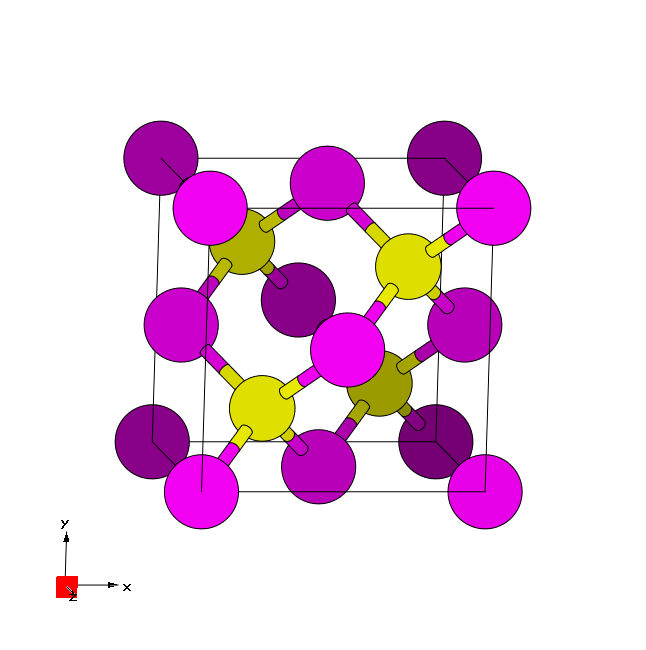
\includegraphics[width=0.25\columnwidth,trim={55pt 55pt 55pt 55pt},clip]{figure/example01/GaAs.png}
\caption{Unit cell of GaAs crystal plotted with the \xcrysden{} program.}
\label{fig21}
\end{figure}

\begin{itemize}
	\item [1-3] These are common to all calculations, and they have already been performed in previous examples. Hence, no results are shown here.  

The space group of GaAs is $F{-}43m$ (sequential  number 276 in the International Tables for Crystallography, Vol. A).
In our example the Ga atom is placed at the origin, whose Wyckoff letter is $a$ and its multiplicity is $4$. The site symmetry group of $a$ is ${-}43m$, which is isomorphous to the full point group of the crystal, also known as $T_d^2$. This is due to the fact that $F{-}43m$ is symmorphic. Hence, $a$ contains 24 symmetry operations (see \Tab{tab21.1}). The As atom is placed at (0.25,0.25,0.25) in fractional coordinates, whose Wyckoff letter is $c$ and its multiplicity is 4. It also contains 24 symmetry operations (see \Tab{tab21.2}). 
\begin{table}[b!]
	\centering
	\captionsetup{width=.5\textwidth}
	\caption{24 symmetry operations for the Wyckoff position $4a$ in $-43m$ \cite{bilbaocrystserver}.}
	\begin{tabular}{@{} |l|l|l|l|l|l| @{}}\toprule[1.5pt]
	x,y,z & -x, -y, z & -x,y,-z & x,-y,-z & z,x,y & z,-x,-y \\
	\hline
	-z,-x,y & -z,x,-y & y,z,x & -y,z,-x & y,-z,-x & -y,-z,x \\
	\hline
	y,x,z & -y,-x,z & y,-x,-z & -y,x,-z & x,z,y & -x,z,-y \\
	\hline
	-x,-z,y & x,-z,-y & z,y,x & z,-y,-x & -z,y,-x & -z,-y,x \\
	\bottomrule[1pt]
	\end{tabular}\label{tab21.1}

	\centering
	\captionsetup{width=.5\textwidth}
	\caption{24 symmetry operations for the Wyckoff position $4c$ in $-43m$ \cite{bilbaocrystserver}.}
	\begin{tabular}{@{} |l|l|l|l| @{}}\toprule[1.5pt]
	x,y,z & -x+1/2,-y+1/2, z & -x+1/2,y,-z+1/2 & x,-y+1/2,-z+1/2  \\ 
	\hline
	z,x,y & z,-x+1/2,-y+1/2 & -z+1/2,-x+1/2,y & -z+1/2,x,-y+1/2  \\
	\hline
	y,z,x & -y+1/2,z,-x+1/2 & y,-z+1/2,-x+1/2 & -y+1/2,-z+1/2,x  \\ 
	\hline
	y,x,z & -y+1/2,-x+1/2,z & y,-x+1/2,-z+1/2 & -y+1/2,x,-z+1/2 \\ 
	\hline 
	x,z,y & -x+1/2,z,-y+1/2 & -x+1/2,-z+1/2,y & x,-z+1/2,-y+1/2 \\
	\hline
	z,y,x & z,-y+1/2,-x+1/2 & -z+1/2,y,-x+1/2 & -z+1/2,-y+1/2,x \\
	\bottomrule[1pt]
	\end{tabular}\label{tab21.2}
\end{table}
The list of site-symmetry operations may be found in the {\tt .sym} file and in the output file {\tt pw2wan.out}. In the latter, the list is in the section relative to the computation of the $D_{mn}$ matrix (see Ref.~\onlinecite{Sakuma}).
\end{itemize}
\clearpage

\subsection*{One $s$-like Wannier function centred at Ga}
\begin{itemize}
	\item[1-5] {\it  Compute the symmetry-adapted MLWF.}

	The ${-}43m$ site-symmetry group is isomorphous to $T_d^2$. From the table of characters of $T_d^2$ we find 5 irreducible representations (\textit{irrep}). The irrep with character $A_1$ is a one-dimensional representation, whose eigenfunction is spherically symmetric. Hence, a single $s$-like orbital in (0,0,0) may be used. However, this is not enough as the choice of the initial guess must also be compatible with the symmetry of the bands. In fact, if we tried to wannierise only the lowest band, excluding all the other bands (this can be done by changing the input file as {\tt num\_wann = 1, num\_bands = 1} and {\tt exclude\_bands = 1-5, 7-19}), the resulting $1\times1$ $U(\mathbf{k})$ could not fulfill Eq. 19 in Ref.~\onlinecite{Sakuma}. Similarly, if we tried to wannierise only the three top bands. 
	{\tt
	\begin{quote}
	begin projections
	
	f= 0.0, 0.0, 0.0 : s
	
	end projections
	\end{quote}
	}
\end{itemize}

 	\begin{tcolorbox}[sharp corners,boxrule=0.5pt]
 	{\small
 	\begin{verbatim}
  ----------------                                                                    
  *** Compute DMN                                                                     
  ----------------                                                                    
                                                                                      
  Number of symmetry operators =    24    
	\end{verbatim}
	}
	\end{tcolorbox}

	\begin{figure}[h!]
	\centering
	\subfloat[Wannier-interpolated band]{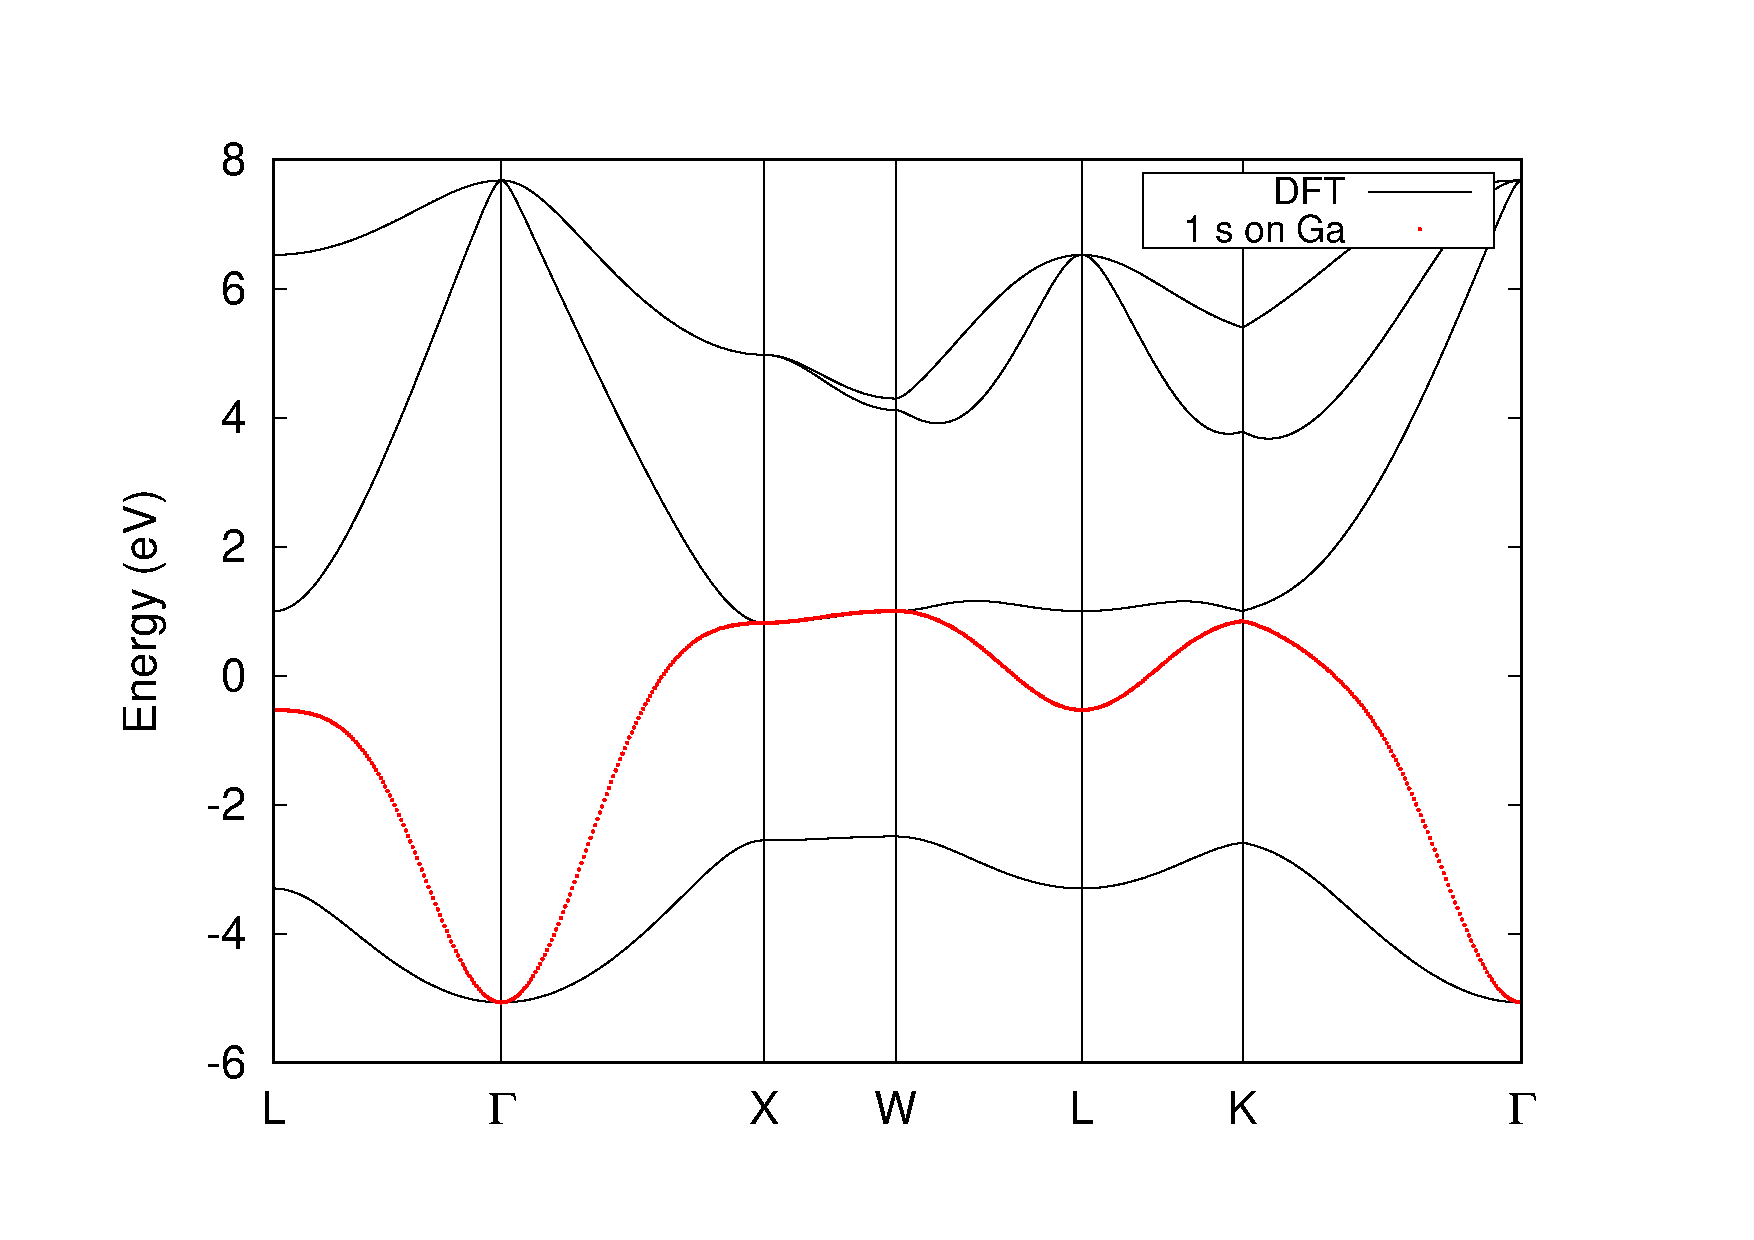
\includegraphics[width=0.6\columnwidth]{figure/example21/GaAs_BS_Ga_s_DFT.pdf}}
	\centering
	\subfloat[Sym.Ad. MLWF]{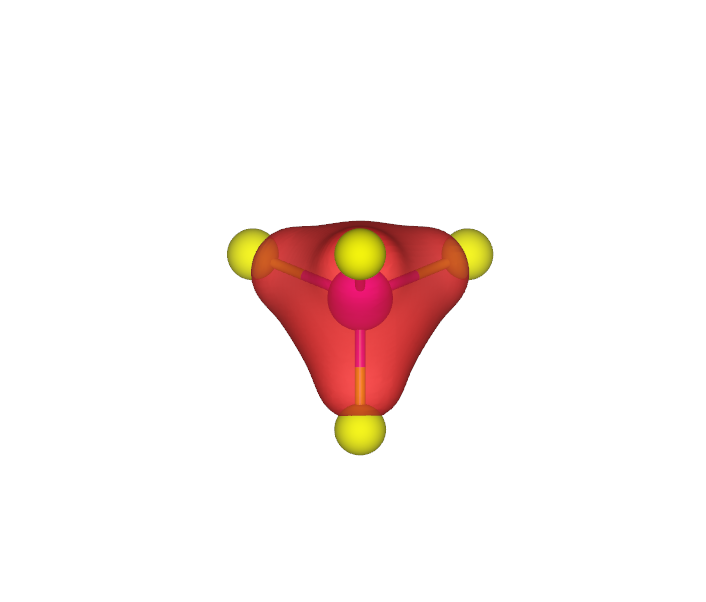
\includegraphics[width=0.2\columnwidth,trim={120pt -70pt 60pt 70pt},clip]{figure/example21/GaAs_Ga_s.png}}
	\caption{One $s$-like symmetry-adapted Wannier function centred on the Gallium atom in GaAs.}\label{fig21.1}
	\end{figure}
\clearpage

\subsection*{Three $p$-like Wannier functions centred at Ga}
\begin{itemize}
	\item[1-5] {\it  Compute the symmetry-adapted MLWFs.}

    Another representation of ${-}43m$, namely $T_2$, has dimension 3. Its eigenfunctions are linear functions proportional to $x,y,z$. Hence, we can use three $p$-like orbitals ($p_x,p_y,p_z$) centred at (0,0,0).
	{\tt
	\begin{quote}
	begin projections
	
	f= 0.0, 0.0, 0.0 : p
	
	end projections
	\end{quote}
	}


\end{itemize}

\begin{figure}[h!]
	\centering
	\subfloat[Wannier-interpolated band]{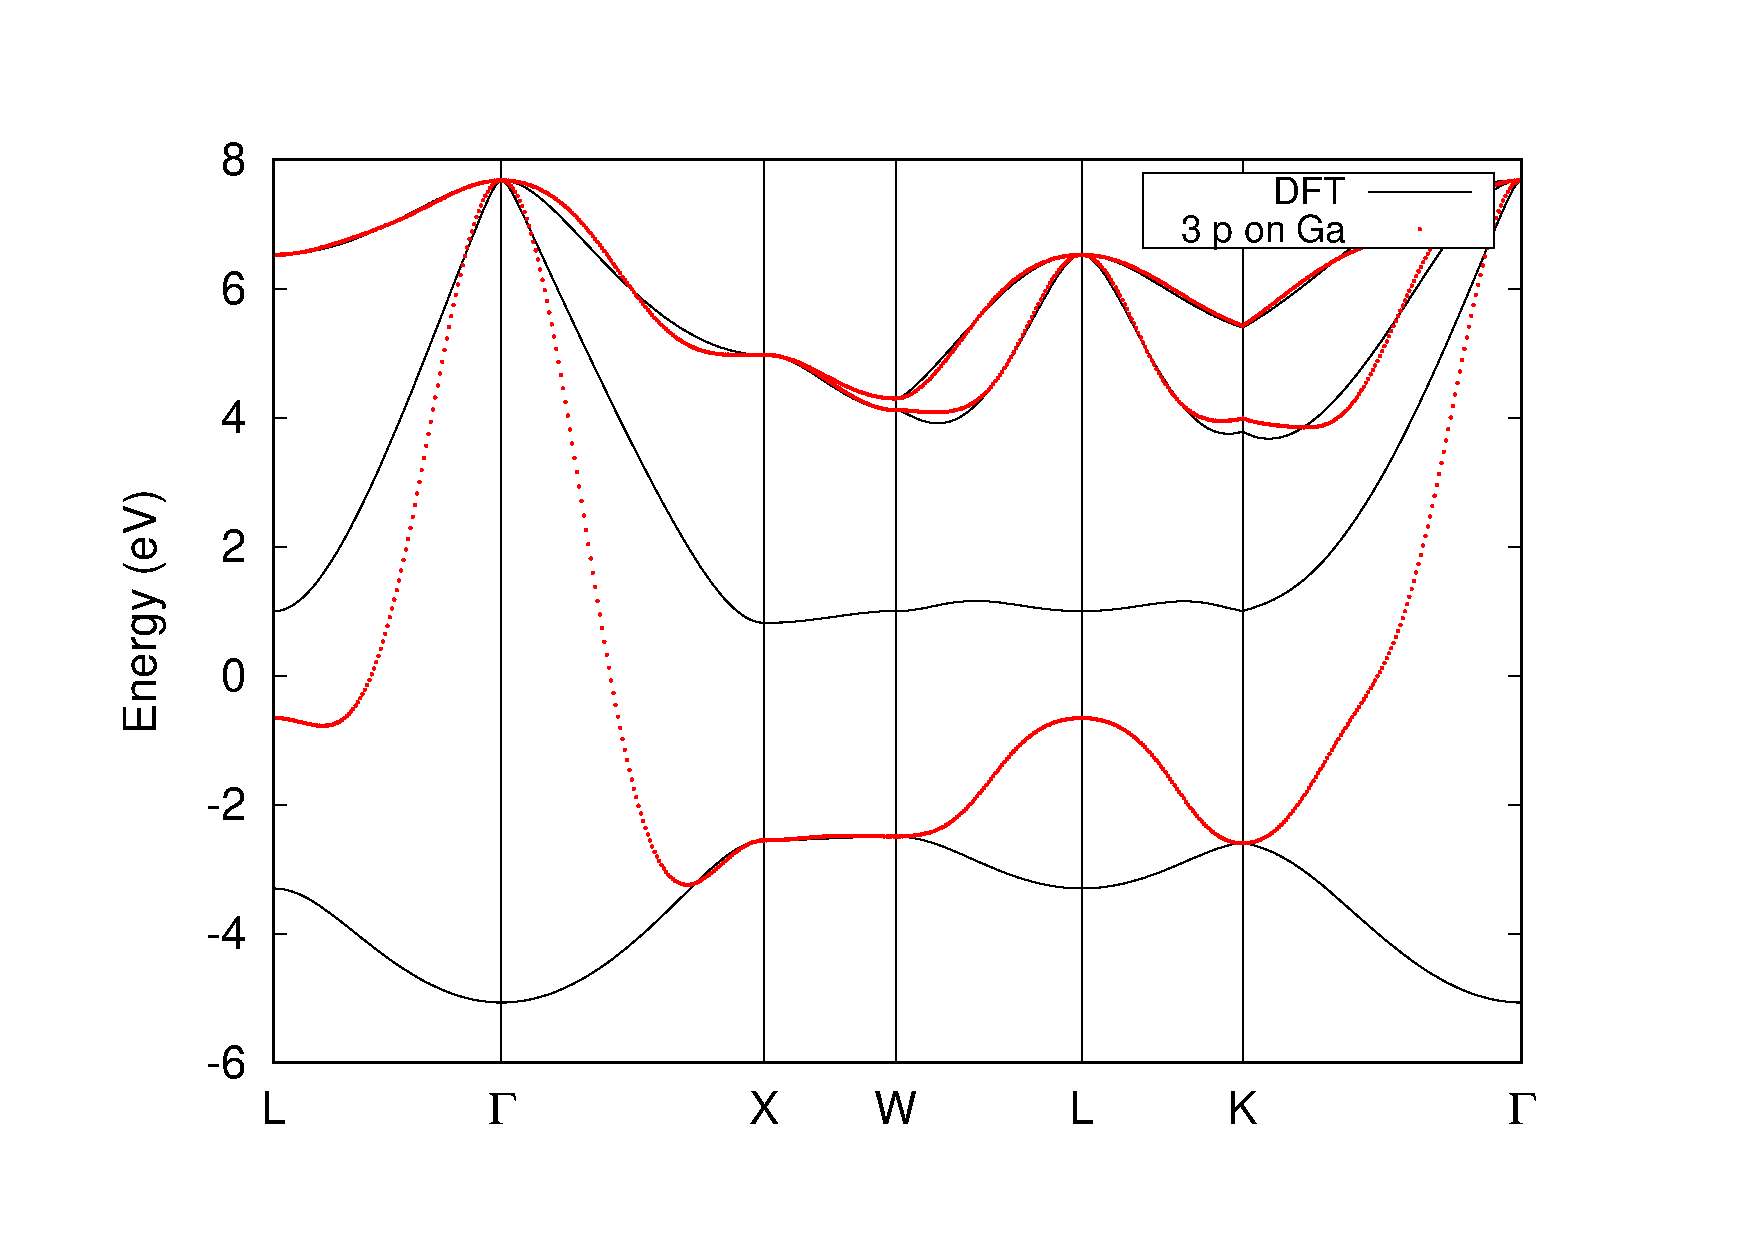
\includegraphics[width=0.6\columnwidth]{figure/example21/GaAs_BS_Ga_p_DFT.pdf}}
	\centering
	\subfloat[Sym.Ad. MLWFs]{\vbox{\offinterlineskip\halign{#\hskip3pt&#\cr
	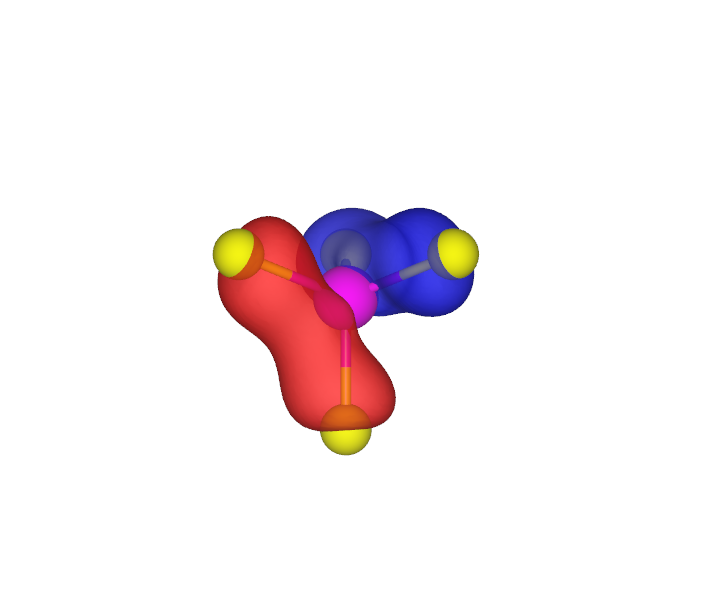
\includegraphics[width=0.2\columnwidth,trim={120pt 70pt 60pt 70pt},clip]{figure/example21/GaAs_Ga_p_p1.png}&
	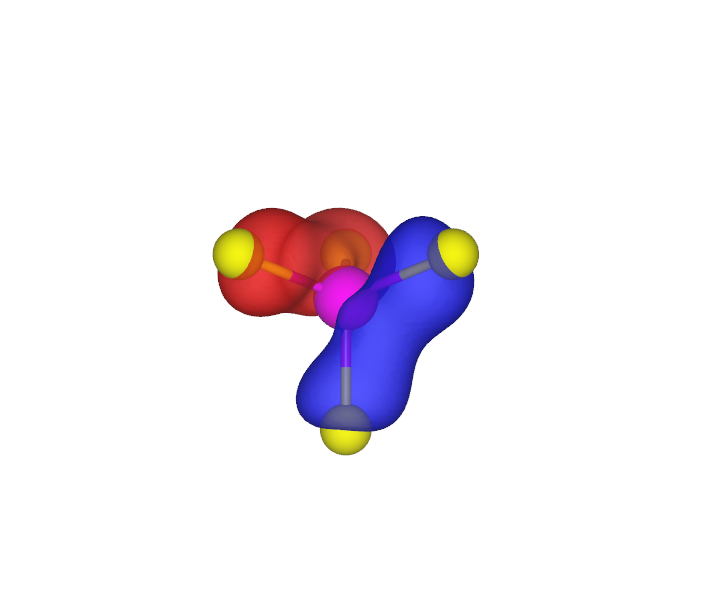
\includegraphics[width=0.2\columnwidth,trim={120pt 70pt 60pt 70pt},clip]{figure/example21/GaAs_Ga_p_p2.png}\cr
	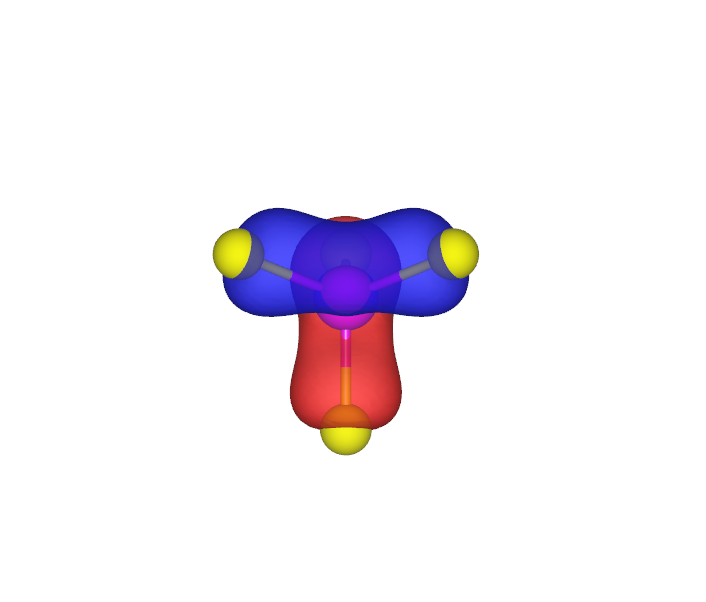
\includegraphics[width=0.2\columnwidth,trim={120pt 70pt 60pt 70pt},clip]{figure/example21/GaAs_Ga_p_p3.png}&
	\cr
	}}}
\caption{Three $p$-like symmetry-adapted Wannier functions centred on the Gallium atom in GaAs.}
\label{fig21.2}
\end{figure}
\clearpage

\subsection*{One $s$-like and three $p$-like Wannier functions centred at Ga}

\begin{itemize}
	\item[1-5] {\it  Compute the symmetry-adapted MLWFs.}

	We can construct also construct a representation of dimension $4=3+1$ for the 4 valence bands by specifying 1 $s$-like orbital and 3 $p$-like orbitals on Ga, which corresponds to the irreducible representations $A_1$ and $T_2$ respectively. However, it would not be possible to  
{\tt
\begin{quote}
begin projections

f= 0.0, 0.0, 0.0 : s

f= 0.0, 0.0, 0.0 : p

end projections
\end{quote}
}

\end{itemize}
	\begin{figure}[h!]
	\centering
	\subfloat[Wannier-interpolated band]{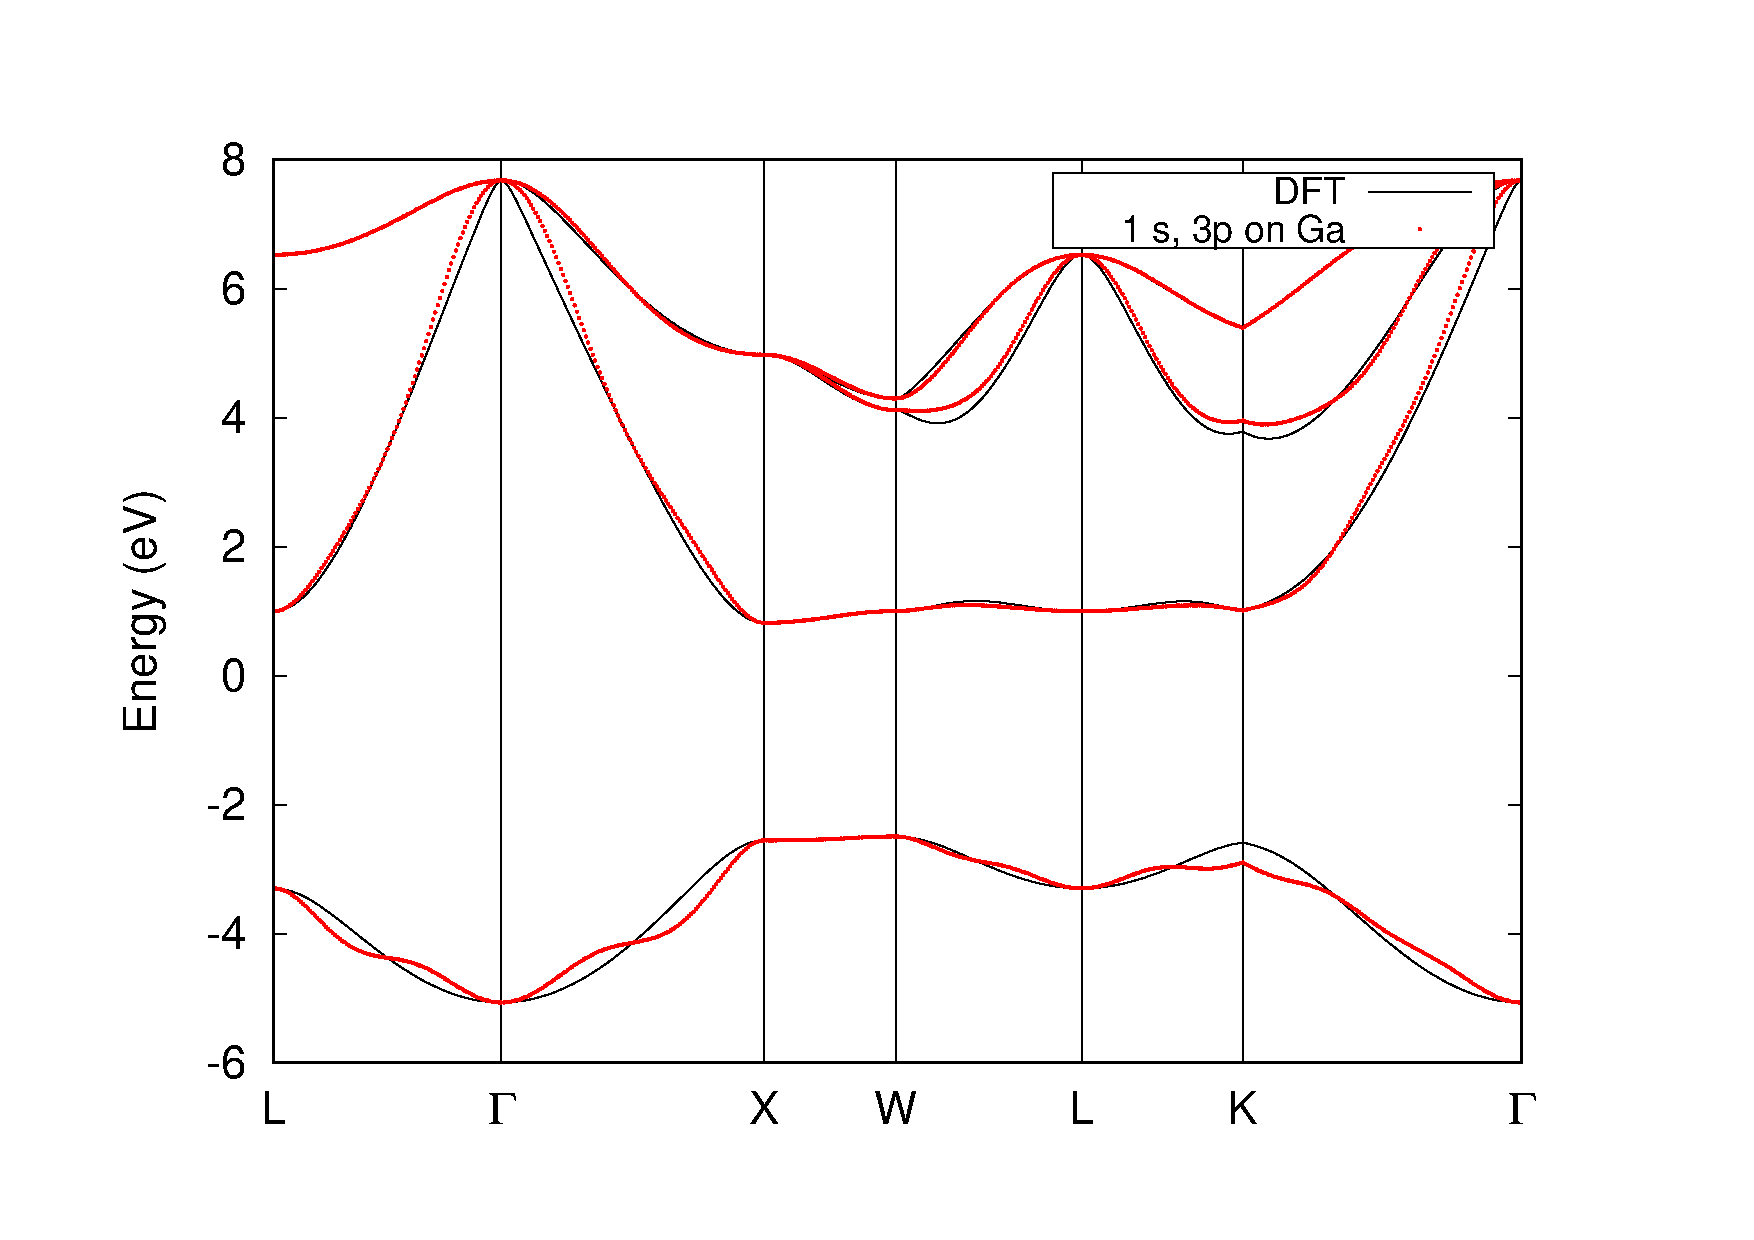
\includegraphics[width=0.6\columnwidth]{figure/example21/GaAs_BS_Ga_sp_DFT.pdf}}
	\subfloat[Sym.Ad. MLWFs]{\vbox{\offinterlineskip\halign{#\hskip3pt&#\cr
	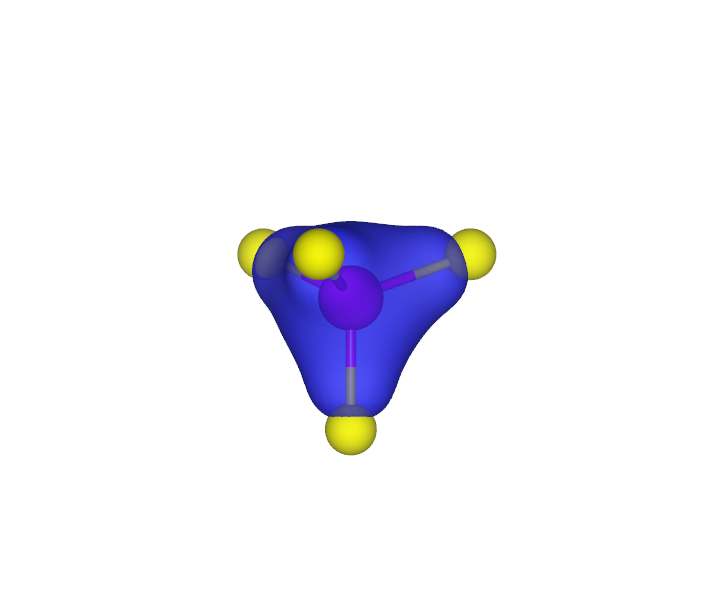
\includegraphics[width=0.2\columnwidth,trim={120pt 70pt 60pt 70pt},clip]{figure/example21/GaAs_Ga_sp_s.png}&
	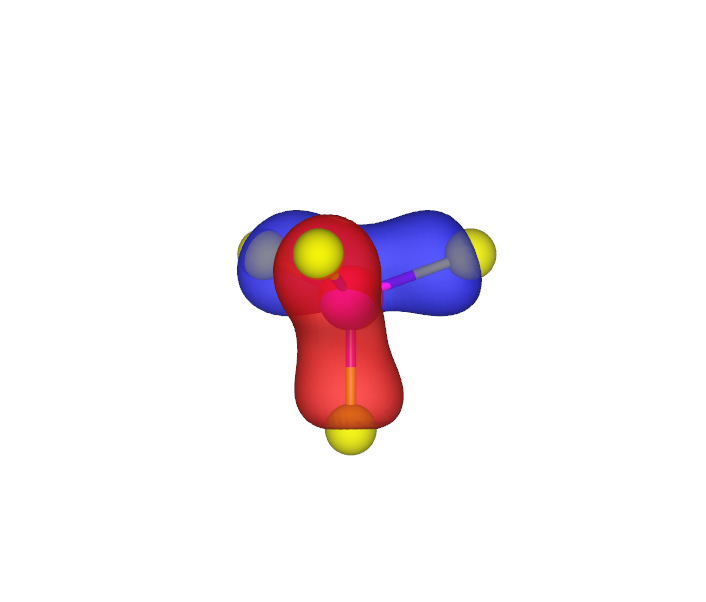
\includegraphics[width=0.2\columnwidth,trim={120pt 70pt 60pt 70pt},clip]{figure/example21/GaAs_Ga_sp_p1.png}\cr
	\noalign{\vskip3pt}
	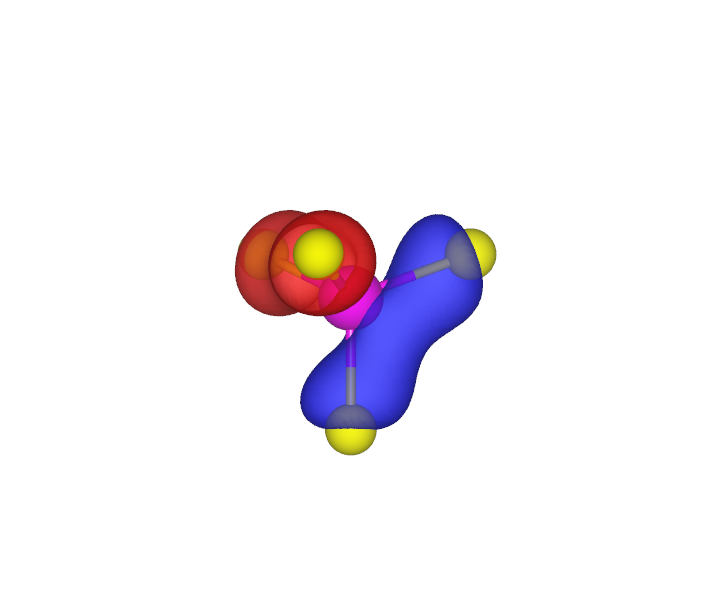
\includegraphics[width=0.2\columnwidth,trim={120pt 70pt 60pt 70pt},clip]{figure/example21/GaAs_Ga_sp_p2.png}&
	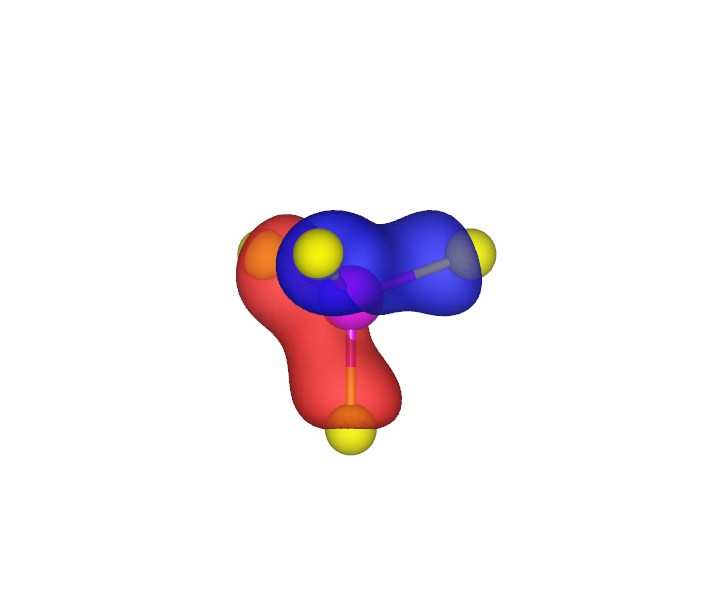
\includegraphics[width=0.2\columnwidth,trim={120pt 70pt 60pt 70pt},clip]{figure/example21/GaAs_Ga_sp_p3.png}\cr
	}}}
	\caption{One $s$-like and three $p$-like Wannier functions centred on the Gallium atom in GaAs.}
	\label{fig21.3}
	\end{figure}

\clearpage

\subsection*{One $s$-like and three $p$-like Wannier functions centred at As}

The site-symmetry group for the As anion centred at $(0.25,0.25,0.25)$ is ${-}43m$ as well and we can perform the same analysis done for the Ga cation. Contrary to the Ga case, for the As anion it is possible to wannierise the bottom band from one $s$-like orbital centred at $(0.25,0.25,0.25)$ and the top three bands from three $p$-like orbitals centred at $(0.25,0.25,0.25)$ (see \Fig{fig21.5}).

\begin{itemize}
	\item[1-5] {\it Compute the symmetry-adapted MLWFs.}

{\tt
\begin{quote}
begin projections

f=0.25,0.25,0.25 : s

f=0.25,0.25,0.25 : p

end projections
\end{quote}
}



\end{itemize}
	\begin{figure}[h!]
	\centering
	\subfloat[Wannier-interpolated band]{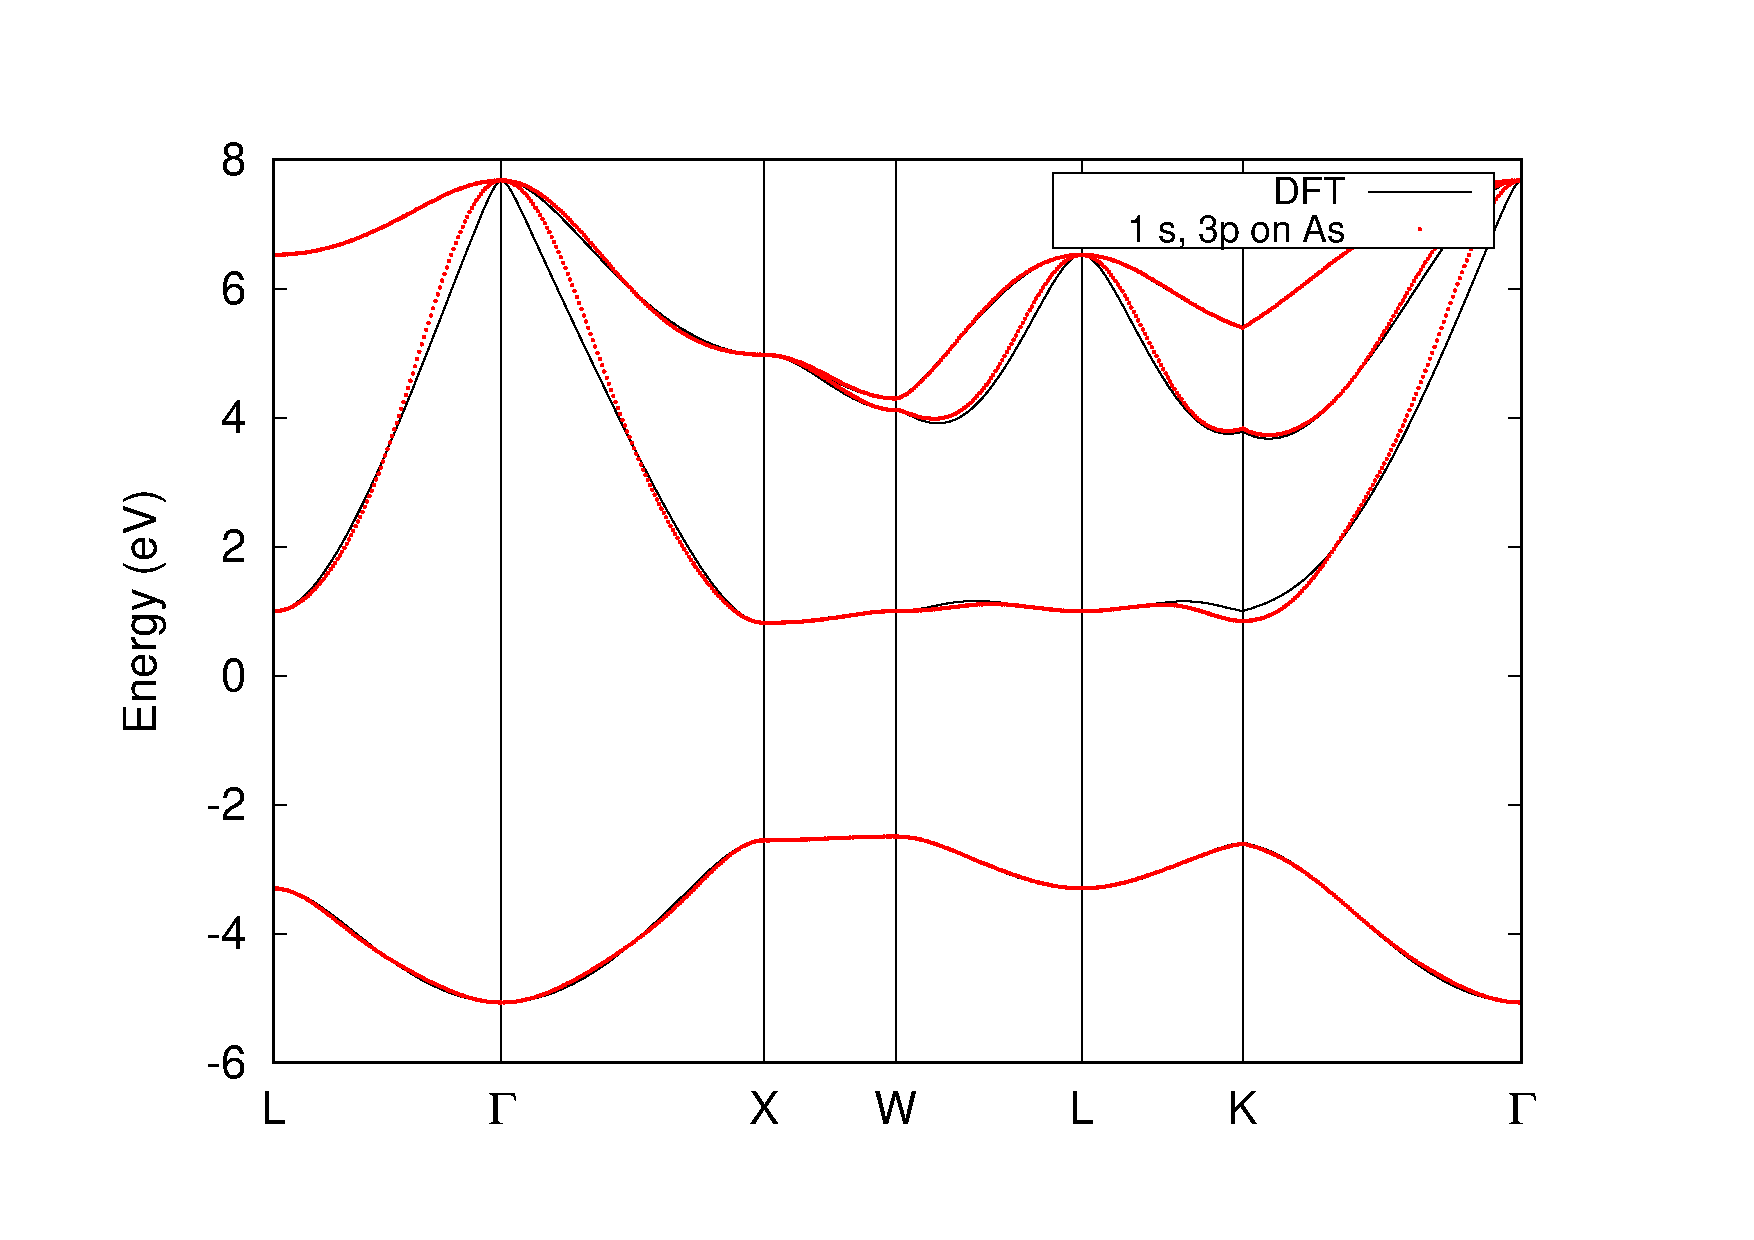
\includegraphics[width=0.6\columnwidth]{figure/example21/GaAs_BS_As_sp_DFT.pdf}}
	\subfloat[Sym.Ad. MLWFs]{\vbox{\offinterlineskip\halign{#\hskip3pt&#\cr
	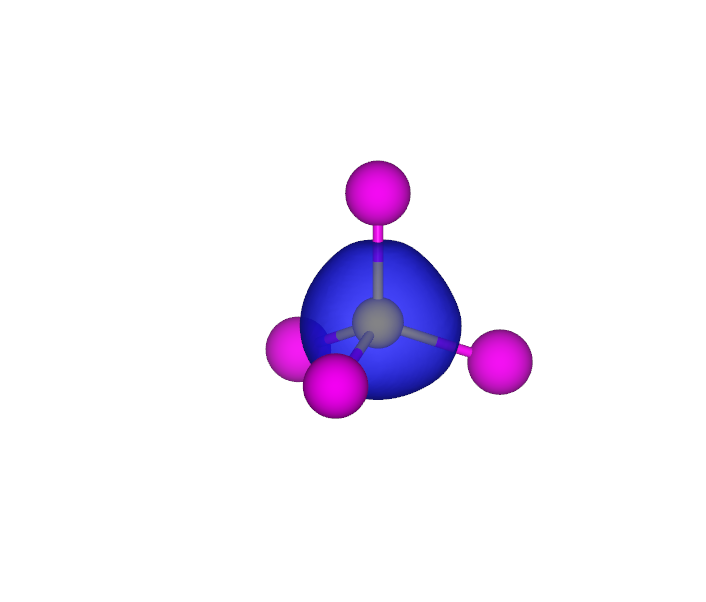
\includegraphics[width=0.2\columnwidth,trim={120pt 70pt 60pt 70pt},clip]{figure/example21/GaAs_As_sp_s.png}&
	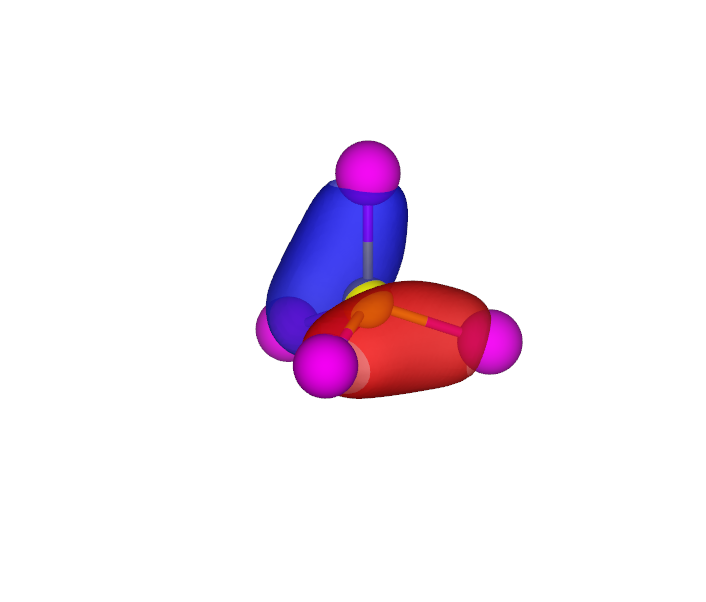
\includegraphics[width=0.2\columnwidth,trim={120pt 70pt 60pt 70pt},clip]{figure/example21/GaAs_As_sp_p1.png}\cr
	\noalign{\vskip3pt}
	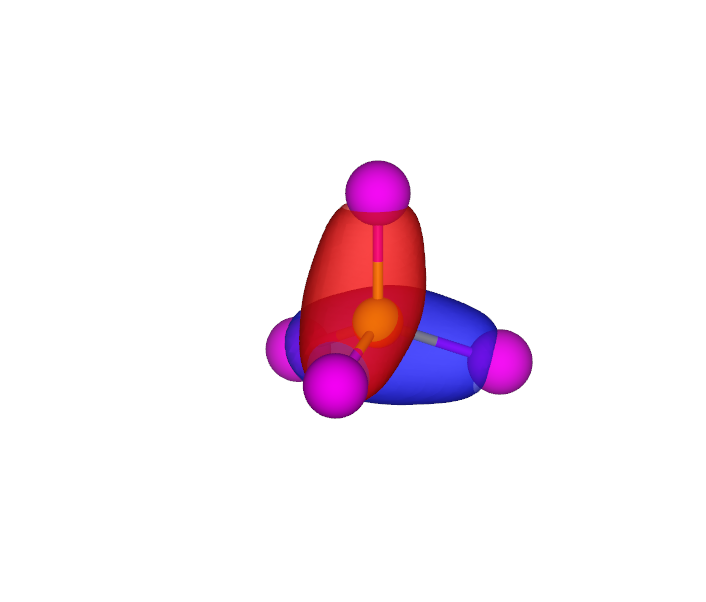
\includegraphics[width=0.2\columnwidth,trim={120pt 70pt 60pt 70pt},clip]{figure/example21/GaAs_As_sp_p2.png}&
	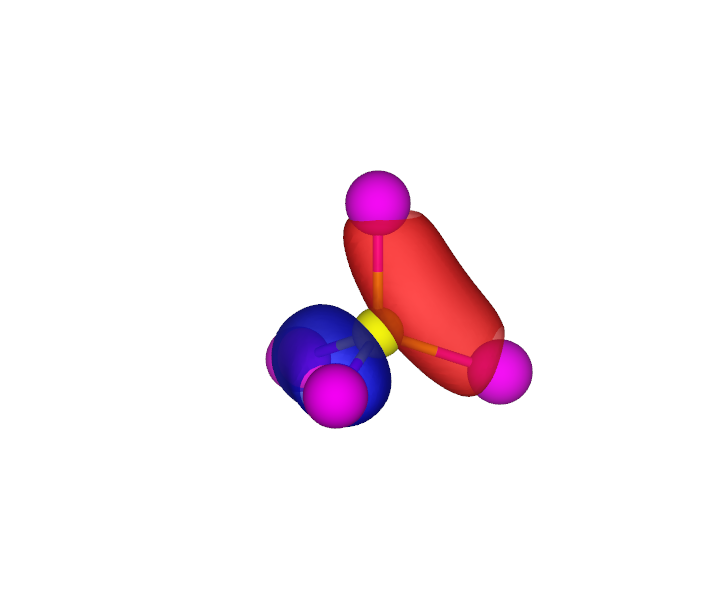
\includegraphics[width=0.2\columnwidth,trim={120pt 70pt 60pt 70pt},clip]{figure/example21/GaAs_As_sp_p3.png}\cr
	}}}
	\caption{One $s$-like and three $p$-like Wannier functions centred on the Arsenic atom in GaAs.}
	\label{fig21.4}
	\end{figure}


	\begin{figure}[h!]
	\centering
	\subfloat[$s$-like orbital on As]{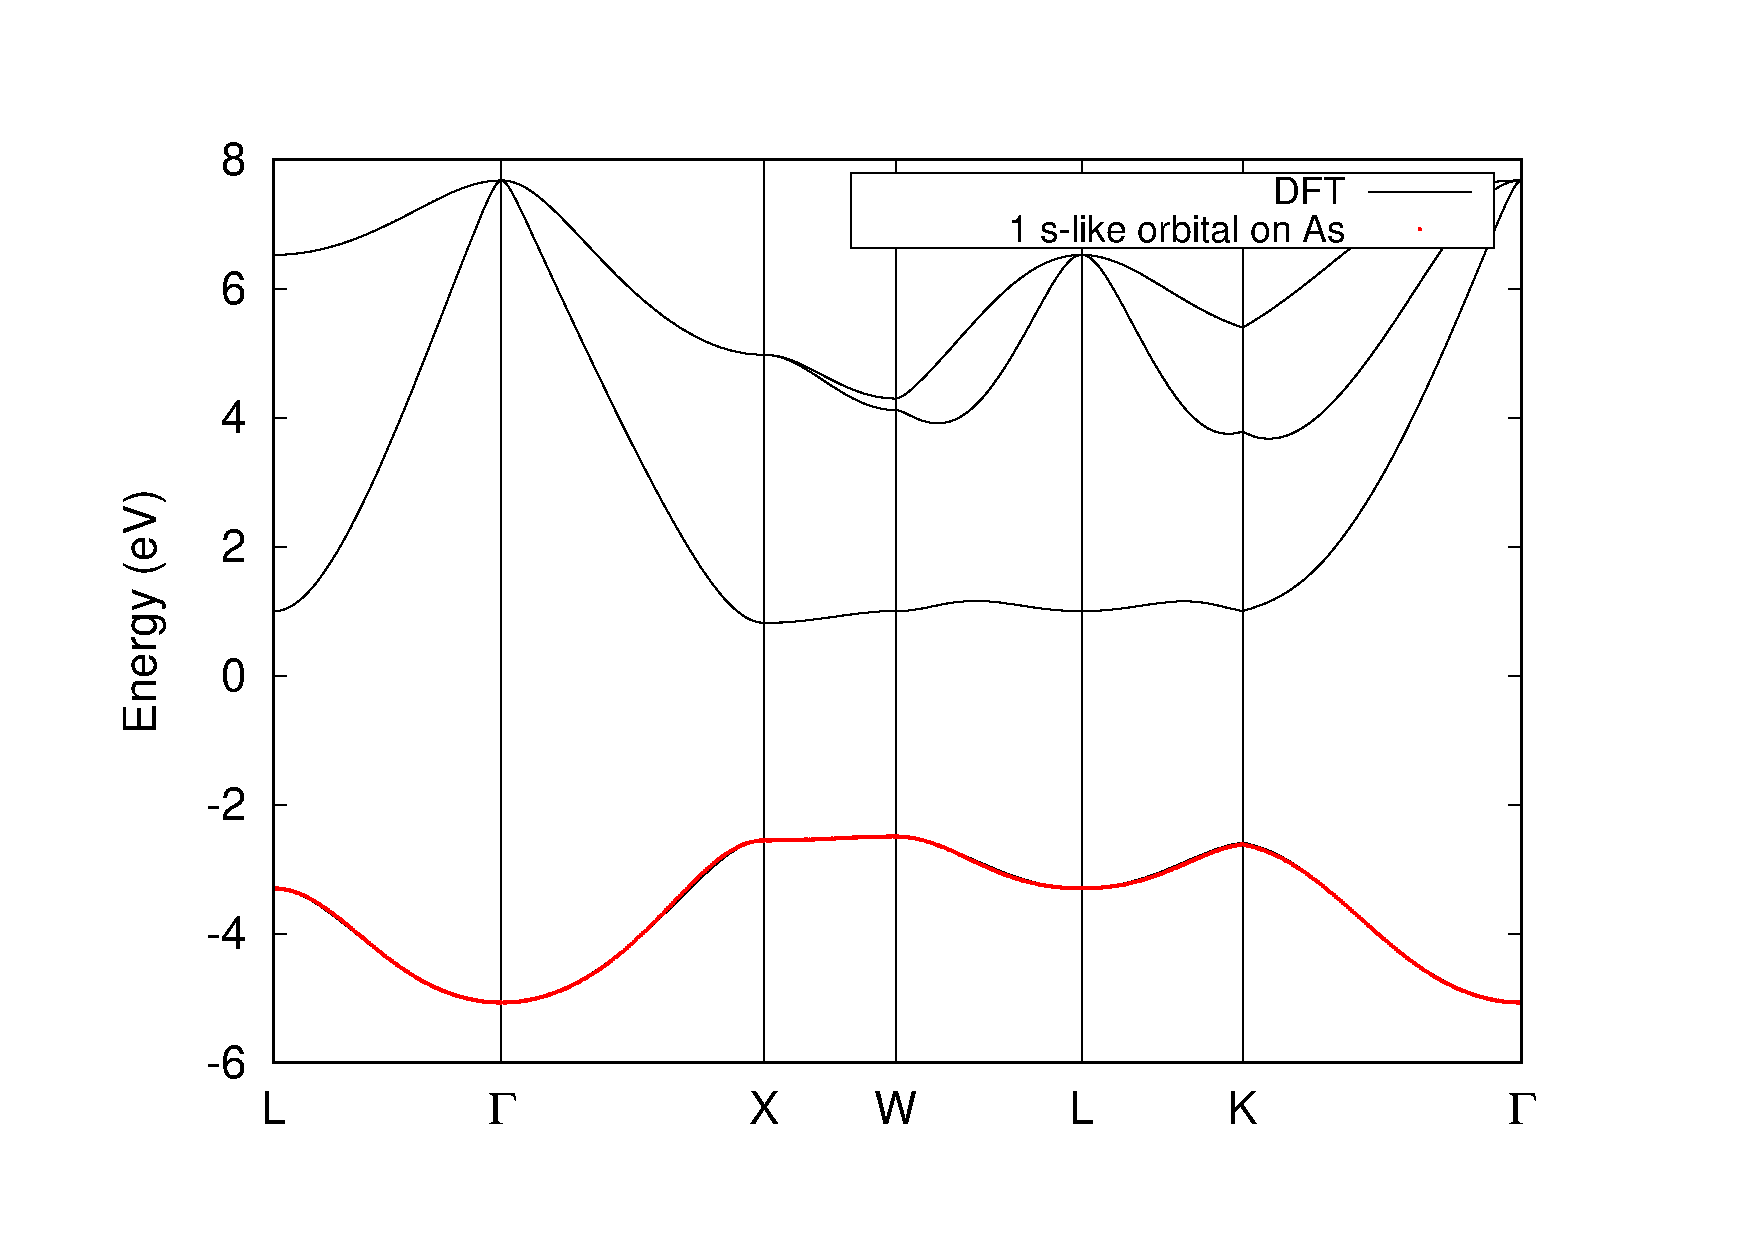
\includegraphics[width=0.7\columnwidth]{figure/example21/GaAs_BS_As_s_DFT.pdf}}\\
	\centering
	\subfloat[3 $p$-like orbitals on As]{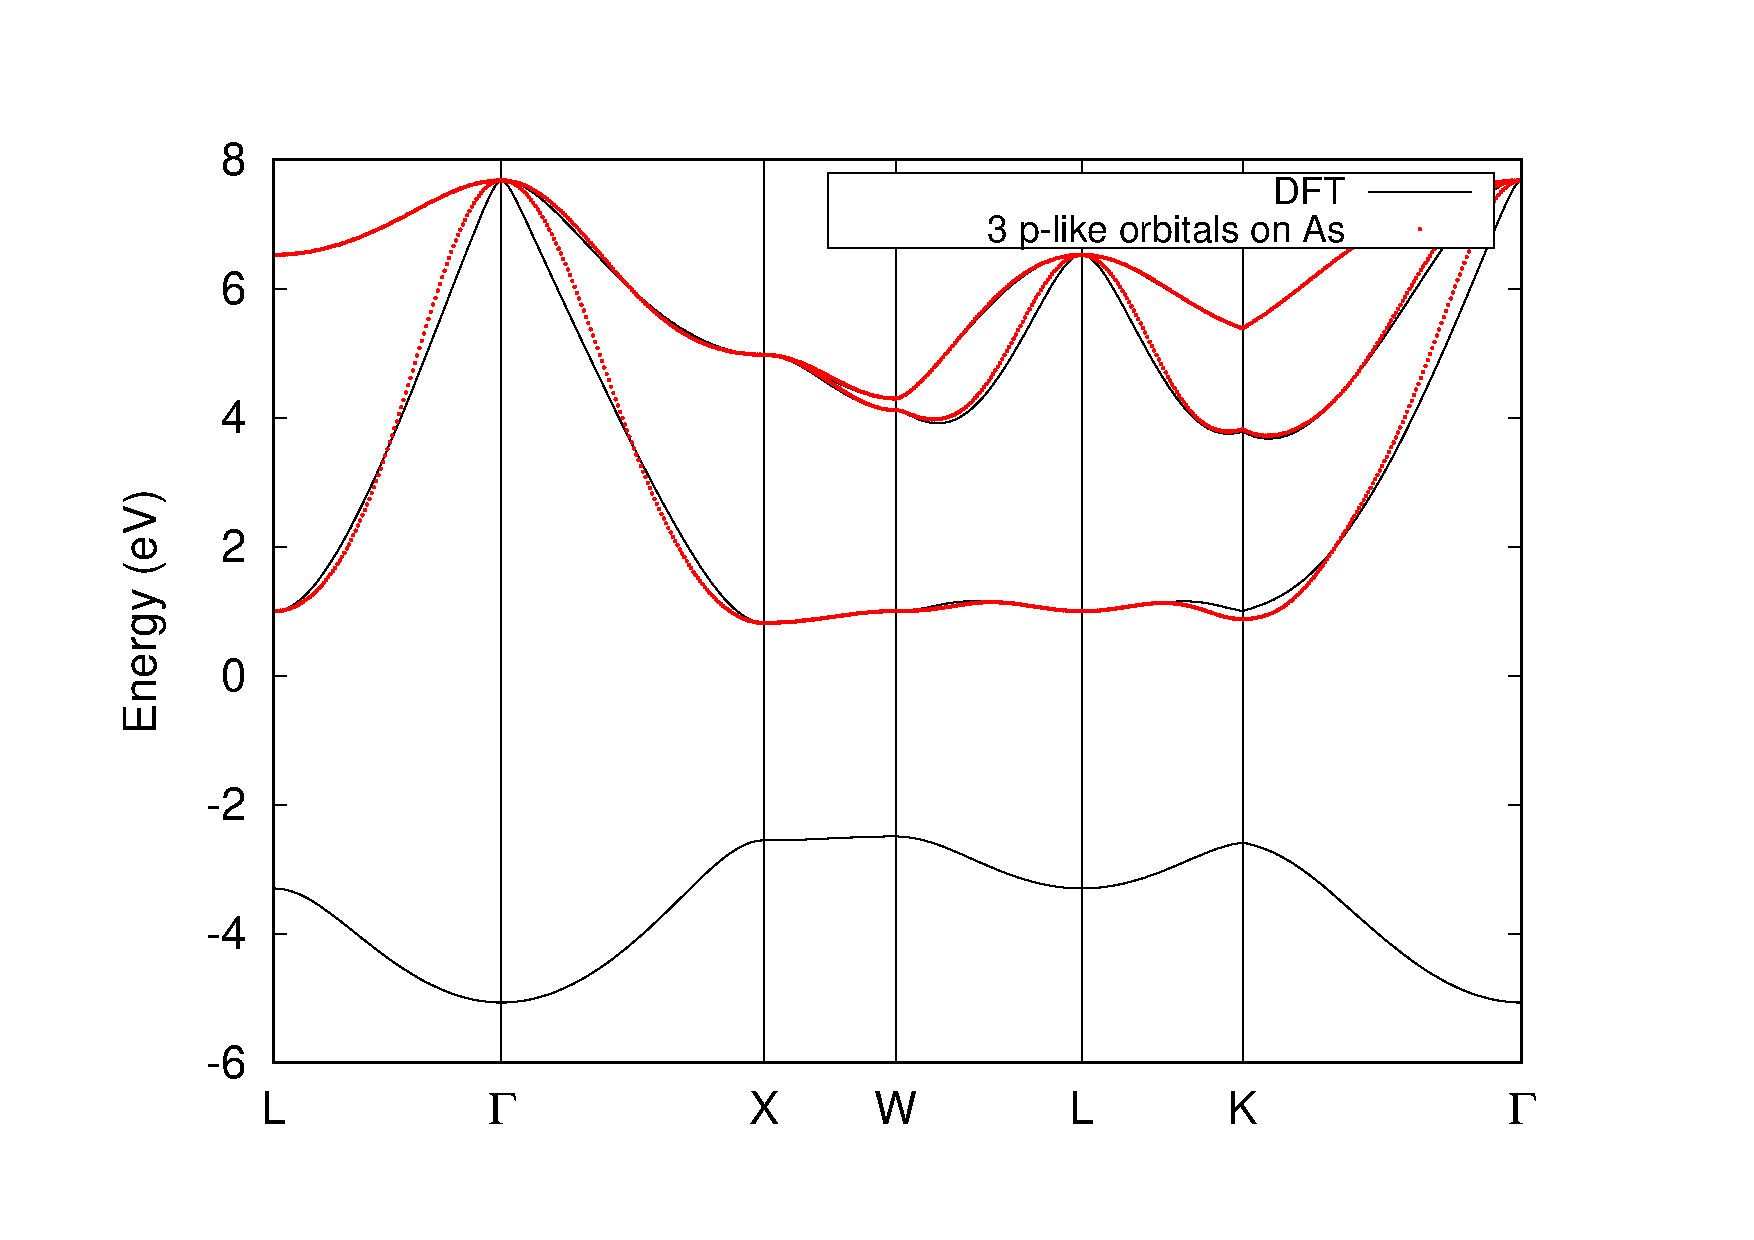
\includegraphics[width=0.7\columnwidth]{figure/example21/GaAs_BS_As_p_DFT.pdf}}
	\caption{Interpolated \Wannier{} bands of GaAs starting from a) 1 $s$-like centred on the Arsenic anion and b) three $p$-like orbitals centred on the Arsenic anion, respectively.}
	\label{fig21.5}
	\end{figure}

\clearpage

\subsection*{Four $s$-like Wannier functions centred on the four Ga-As bonds}

From a group-theoretical point of view, the case of four $s$-like functions centred on four covalent bonds, correspond to the \textit{irrep} $A_{1g}$ of the site-symmetry group $.3m$ of the Wyckoff position $e$. There are 6 symmetry operations for each equivalent position (0.125, 0.125, 0.125), (0.125, 0.125, -.375), (-.375, 0.125, 0.125) and (0.125, -.375, 0.125). The combined 24 symmetry operations turn out to be exactly that of the full ${-}43m$ group.

\begin{itemize}
	\item[1-5] 	{\it  Compute the symmetry-adapted MLWFs.}

	{\tt
	\begin{quote}
	begin projections

f= 0.125, 0.125, 0.125: s

f= 0.125, 0.125, -.375: s

f= -.375, 0.125, 0.125: s

f= 0.125, -.375, 0.125: s

end projections
	\end{quote}
	}
	
\end{itemize}
	\begin{figure}[h!]
	\centering
	\subfloat[Wannier-interpolated band]{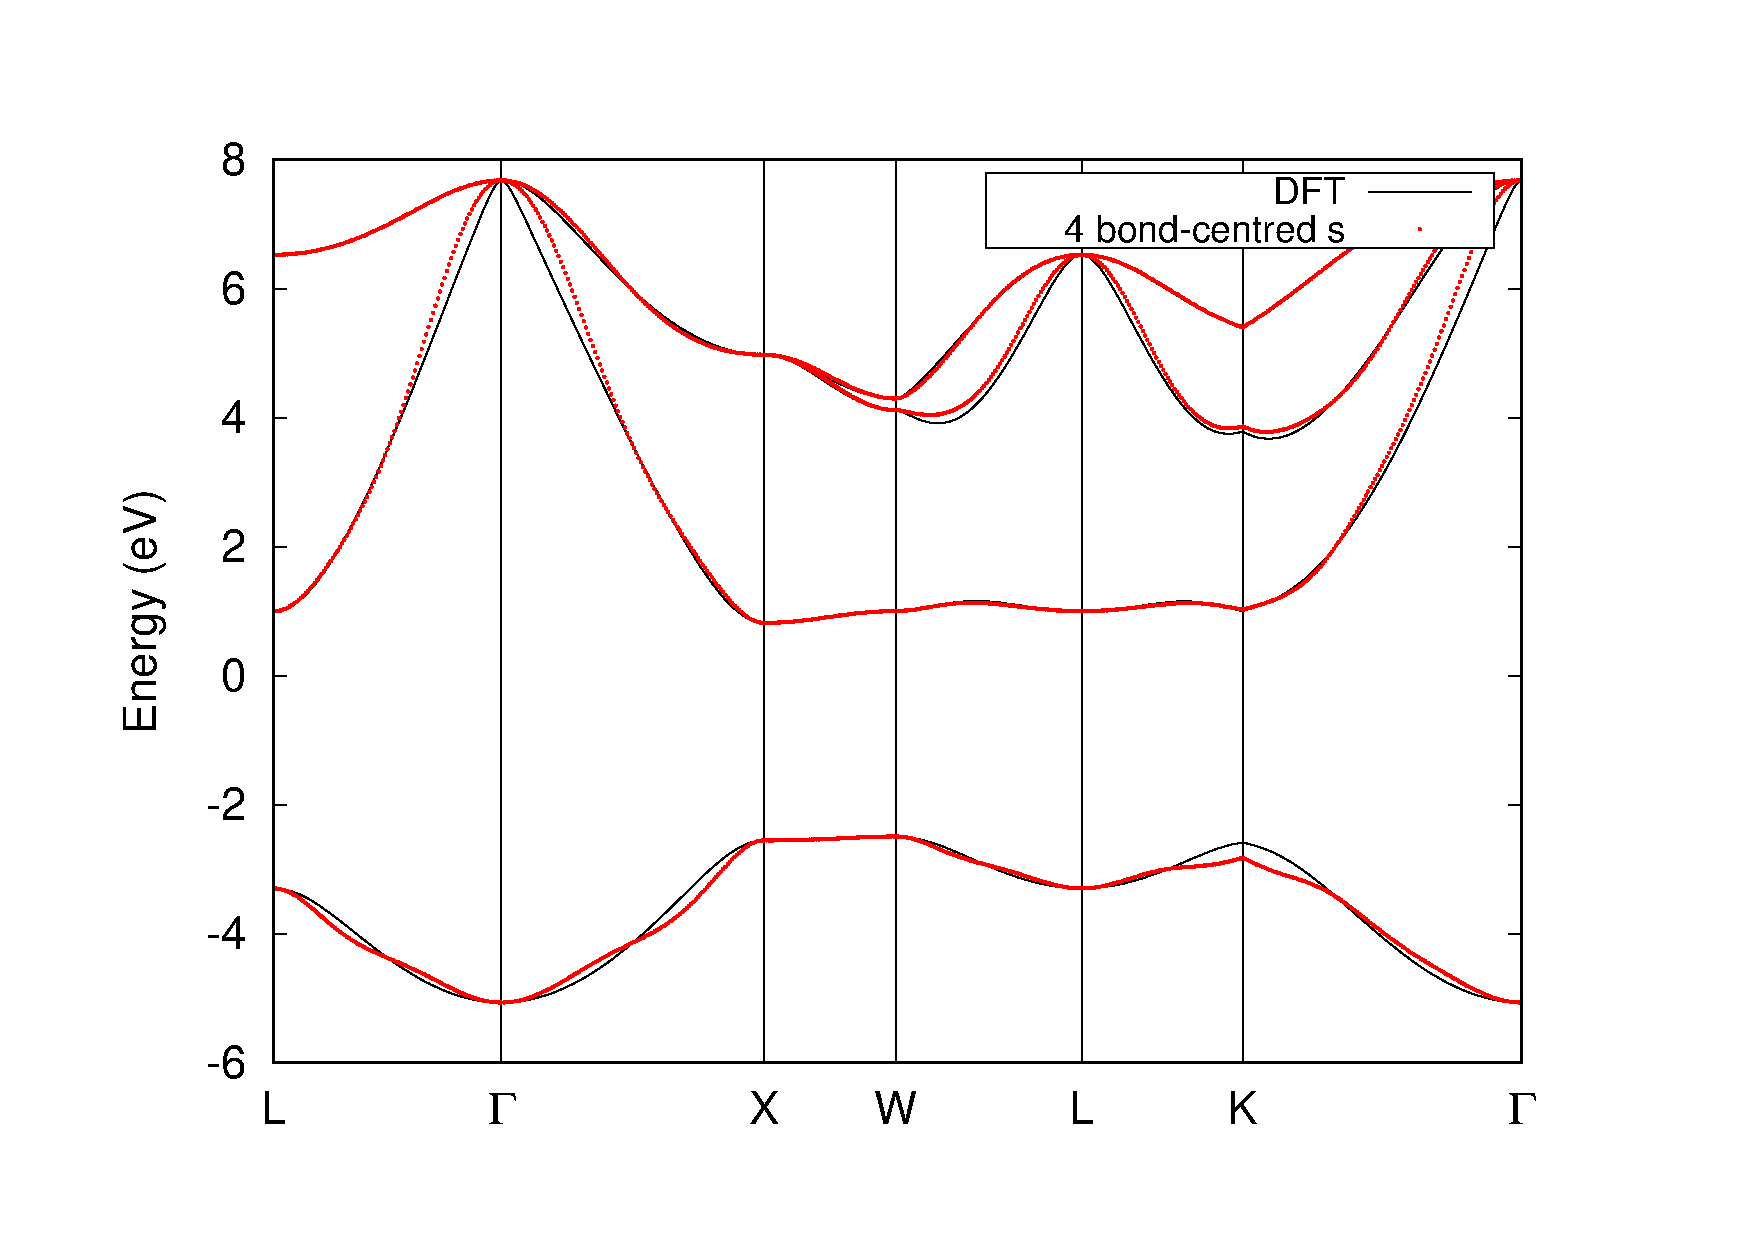
\includegraphics[width=0.6\columnwidth]{figure/example21/GaAs_BS_bond_DFT.pdf}}
	\subfloat[$s,p_x,p_y,p_z$]{\vbox{\offinterlineskip\halign{#\hskip3pt&#\cr
	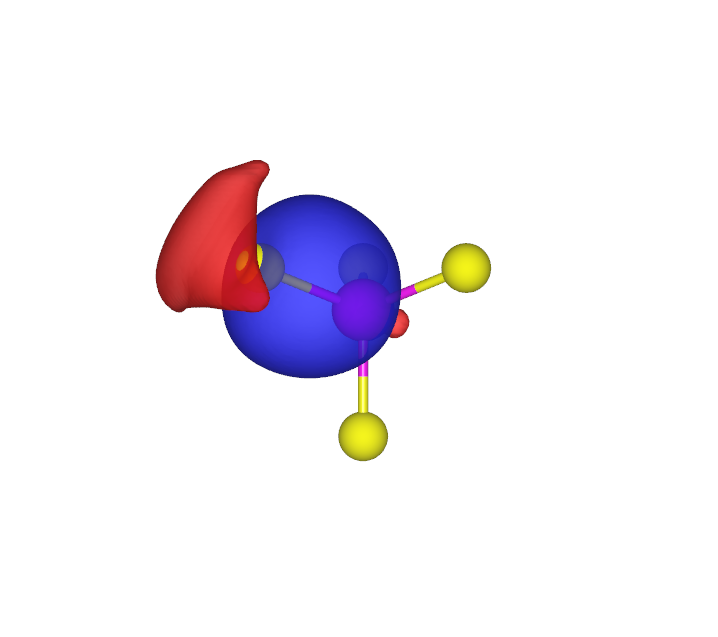
\includegraphics[width=0.2\columnwidth,trim={90pt 80pt 70pt 80pt},clip]{figure/example21/GaAs_bond_sp3_1.png}&
	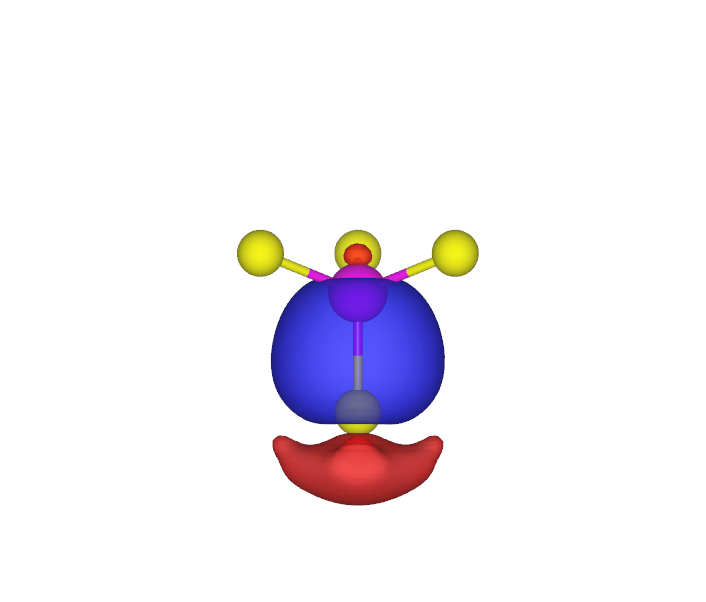
\includegraphics[width=0.2\columnwidth,trim={120pt 70pt 60pt 70pt},clip]{figure/example21/GaAs_bond_sp3_2.png}\cr
	\noalign{\vskip3pt}
	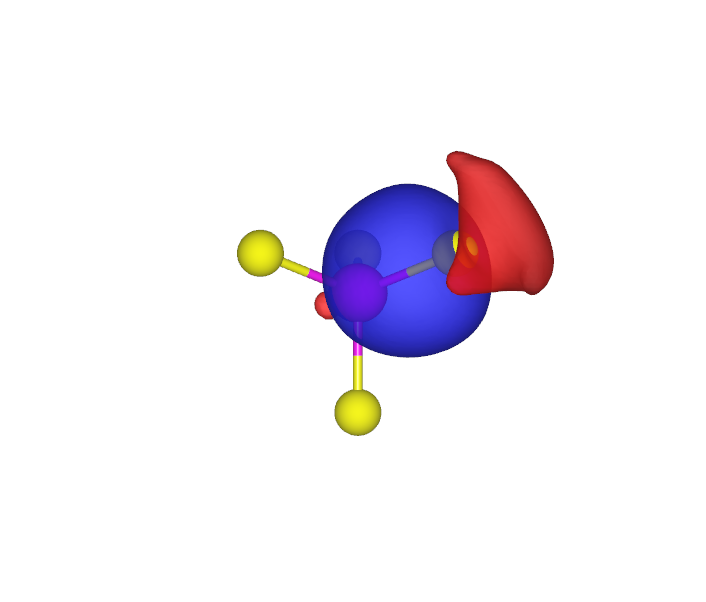
\includegraphics[width=0.2\columnwidth,trim={120pt 70pt 60pt 70pt},clip]{figure/example21/GaAs_bond_sp3_3.png}&
	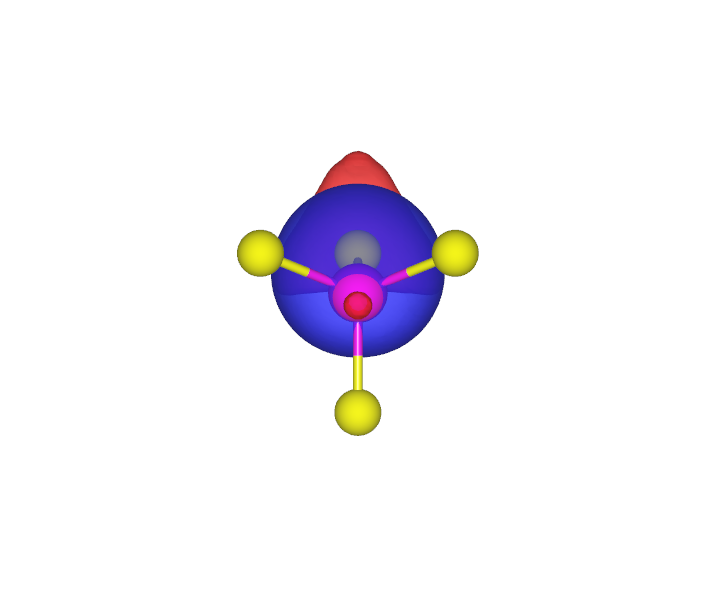
\includegraphics[width=0.2\columnwidth,trim={120pt 70pt 60pt 70pt},clip]{figure/example21/GaAs_bond_sp3_4.png}\cr}}}
	\caption{Four $sp_3$-like symmetry-adapted Wannier functions centred on the Ga-As bonds in GaAs.}
	\label{fig21.6}
	\end{figure}
